\documentclass[crop,tikz]{standalone}% 'crop' is the default for v1.0, before it was 'preview'
\usepackage{tikz,calc,pgfplots}
\usepackage{tikz-3dplot}
\usetikzlibrary{calc}
\usetikzlibrary{calc,patterns,decorations.pathmorphing,decorations.markings}
\usetikzlibrary{shapes.geometric}
\begin{document}


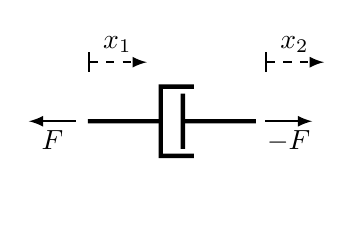
\begin{tikzpicture}[scale=1.5,xshift=0.5cm,every node/.style={outer sep=0pt,thick}]
	
	
	\tikzstyle{spring}=[ultra thick,decorate,decoration={zigzag,pre length=0.4cm,post length=0.5cm,segment length=6}]
	
	\tikzstyle{damper}=[ultra thick,decoration={markings,  
		mark connection node=dmp,
		mark=at position 0.5 with 
		{
			\node (dmp) [ultra thick,inner sep=0pt,transform shape,rotate=-90,minimum width=25pt,minimum height=8pt,draw=none] {};
			\draw [ultra thick] ($(dmp.north east)+(4pt,0)$) -- (dmp.south east) -- (dmp.south west) -- ($(dmp.north west)+(4pt,0)$);
			\draw [ultra thick] ($(dmp.north)+(0,-10pt)$) -- ($(dmp.north)+(0,10pt)$);
		}
	}, decorate]
	
	\tikzstyle{ground}=[draw=none,minimum width=2.5cm,minimum height=0.3cm]


	\node (wall1) at (0.5cm,-2cm) [ground, rotate=90, minimum width=1.5cm] {};
	\node (u0) at (wall1.south) [right,xshift=-0.9cm,yshift=-1cm] {$\phantom{x_2=0}$};

	
	\node (wall1) at (0.5cm,-2cm) [, rotate=90, minimum width=1.5cm] {};
%	\draw [ultra thick] (wall1.north east) -- (wall1.north west);
	\draw [damper] (-1cm,-2cm) -- (wall1.north) node[] {};
	
	\draw [latex-, thick] (-1.5cm,-2cm) --  ++(0.4cm,0cm) node[pos=.5,,below] {$F$};
	\draw [-latex, thick]  (0.5cm,-2cm) --  ++ (0.4cm,0cm) node[pos=.5,below] {$-F$};
	\draw [|-latex, thick,dashed] (-1cm,-1.5cm) -- (-0.5cm,-1.5cm) node[above,midway] {$x_1$};
	\draw [|-latex, thick,dashed] (0.5cm,-1.5cm) -- (1cm,-1.5cm) node[above,midway] {$x_2$};	
	
\end{tikzpicture}

\end{document}